\documentclass[acmsmall,screen,review]{acmart}
\usepackage{booktabs}
\usepackage{siunitx}
\setcopyright{none}
\acmJournal{TOS}

\begin{document}

\title{How KV Dies Decides How Flash Wears:\texorpdfstring{\\}{ }
Endurance and Provisioning of Hybrid CXL Memory for LLM KV Caches}

\author{Romyull Islam}
\email{mislam22@students.kennesaw.edu}
\affiliation{%
  \institution{Kennesaw State University}% department to be added
  \city{Kennesaw}
  \state{Georgia}
  \country{USA}}

\begin{abstract}
Flash is becoming a tier of the LLM key-value (KV) cache: NVIDIA's context memory platform adds a
pod-level flash tier for KV, an SSD vendor has announced an SSD platform for KV caching rated at 7 to
more than 10 effective drive writes per day, and hybrid CXL memory devices put a DRAM cache in front of
a terabyte or more of NAND as memory-attached capacity. Whether that flash lasts depends on how much
KV a node writes and how the flash translation layer amplifies it. Prior hybrid CXL designs
evaluate latency and throughput, and flash-wear studies of KV target on-package high-bandwidth flash,
and most assume write amplification 1; we found no study of how long a hybrid CXL device lasts as a KV
cache, or of what to provision so that it lasts. We answer with six
production traces from two providers (chat, API, coding, reasoning and agent traffic), a model of
a hybrid device scaled consistently to the prefill throughput of one 8-GPU node, and a flash
translation layer validated against closed forms and the MQSim simulator. Three findings stand out.
First, how KV dies decides how flash wears: an LRU prefix cache evicts in near write order and keeps
write amplification near 1 (median 1.00, at most 1.94 at 7\% over-provisioning), while KV freed per request
interleaves lifetimes and reaches 2.1 with TRIM and 5.2 without it at 7\% over-provisioning, the
case on CXL.mem, which has no TRIM. Second, the write rate itself is the wall: without admission control a node at full prefill
duty writes 280 to 1,290\,TB of BF16 KV to flash per day; with second-hit admission, TLC lasts five
years in only 10 of 108 cases, mostly API-like traffic at partial prefill duty and an MLA model with
4-bit KV at partial duty; other traffic needs pseudo-SLC or SLC, and 20 of the 108 cases exceed
even SLC.
Third, the cheap levers are admission control and KV precision (FP8 and INT4 halve and quarter the
writes, about one flash class each); device DRAM changes the NAND writes of a prefix cache little.
For request-scoped KV, a discard command per finished request, sent on the slow management path,
lets the device drop dead KV from its DRAM and trim it, cutting flash writes 3.4 to 9.1 times. We
turn these results into provisioning rules across flash type, KV precision, admission and prefill
duty, and show that a shared pool beats load-balanced, cache-aware routing by only 1 to 18\%.
\end{abstract}

\begin{CCSXML}
<ccs2012>
<concept><concept_id>10010583.10010600.10010607</concept_id>
<concept_desc>Hardware~Non-volatile memory</concept_desc><concept_significance>500</concept_significance></concept>
<concept><concept_id>10010520.10010521</concept_id>
<concept_desc>Computer systems organization~Architectures</concept_desc><concept_significance>300</concept_significance></concept>
</ccs2012>
\end{CCSXML}
\ccsdesc[500]{Hardware~Non-volatile memory}
\ccsdesc[300]{Computer systems organization~Architectures}
\keywords{CXL, hybrid memory, NAND flash, endurance, write amplification, KV cache, LLM serving}

\maketitle

\section{Introduction}
Long contexts, multi-turn chat and agents make LLM serving reuse large prefixes, and serving
systems keep the KV cache of those prefixes beyond GPU memory to avoid recomputing
them~\cite{mooncake,lmcache,kvwild}. The tier below host memory is increasingly flash. NVIDIA
Dynamo's KV block manager offloads KV from GPU memory to host memory and on to local
SSDs~\cite{dynamo_kvbm}, and NVIDIA's CMX context memory platform adds a pod-level,
Ethernet-attached flash tier built for KV~\cite{nvidia_cmx}. Vendors already see wear as the limit:
ScaleFlux has announced an SSD platform for KV caching rated at 7 to more than 10 effective drive
writes per day (DWPD), against 1 to 3 for mainstream TLC drives, and reports that KV blocks with different
lifetimes sharing flash blocks raise write amplification, which lifecycle-aware placement more than
halved in preliminary tests~\cite{scaleflux}. Whether 10 DWPD is enough, and for which traffic,
has no public answer. CXL lets a server attach memory next to its GPUs. Hybrid CXL devices such as
Samsung's CMM-H put a DRAM cache of 16 to 48\,GB in front of a terabyte or more of NAND
flash~\cite{cmmh,cmmh_hs}, and several recent systems build KV caches on CXL-attached flash:
HyMCache~\cite{hymcache}, ITME~\cite{itme}, LM-CXD~\cite{lmcxd} and TempoKV~\cite{tempokv}. They
report time to first token and throughput, and HyMCache and ITME also report hit rates. None
measures wear: HyMCache and TempoKV never discuss endurance, ITME discusses it only qualitatively,
and LM-CXD aligns KV chunks with erase blocks to avoid garbage collection without quantifying wear.

Flash wears out after about 1,000 program/erase cycles for TLC~\cite{cai_proc}. A KV cache writes every block it
admits, and an LLM node computes new KV at gigabytes per second. Whether a hybrid device can absorb
that stream for its rated lifetime is the first question a device maker or an operator has to
answer. Recent work on on-package high-bandwidth flash (HBF) answers parts of it: on the
Qwen-Bailian traces a flash KV tier writes 1.14 to 4.90 times more than it reads, 48 to 140\,TB
per day per eight-GPU system, against a 21.7\,TB/day TLC budget at write amplification
1~\cite{hbfsucks}; KV pages with different lifetimes mixed in one erase block drive
garbage-collection write amplification to about 30 on average for one model~\cite{hbflex};
lifetime-aware placement~\cite{hbflex,lachesis}, cache admission (for recommendation
KV)~\cite{huawei_hbf} and request admission~\cite{berkeley_hbf} extend HBF life; whether HBF
endurance suffices depends on the KV read-to-write ratio~\cite{son_hbf,kyung_hbf}; and TRIM has
been argued for CXL memory in general~\cite{trimcxl}. None of this models a
DRAM-over-NAND CXL device, contrasts the ways KV dies, sweeps flash type and KV precision, or
divides the device among the interleaved streams of a node.

This paper answers the question for hybrid CXL devices and turns the answer into provisioning
rules. The write rates per node and the effect of how KV dies apply to other flash KV tiers
serving the same traffic; one result is specific to CXL: CXL.mem carries neither TRIM nor the placement hints of NVMe
flexible data placement, so the device cannot learn which KV is dead or which KV dies together.
We ask three questions. How much KV does a serving node write to flash per day? What decides write
amplification for KV? And which flash class, KV precision and admission policy let a device last
five years? The answers in brief: hundreds of terabytes per day without admission control; how KV
dies; and a device rated 10 DWPD covers only 40 of our 108 cases with second-hit admission, 9 of 54
for a dedicated prefill node. We make five contributions.
\begin{itemize}
\item A trace-driven model of a hybrid device (DRAM cache over NAND, three admission policies) with
consistent per-node scaling: one node is modeled as $S$ interleaved copies of a trace, with $S$
chosen so that the traffic fills the node's prefill compute at duty $d$, and the device divided accordingly
(Section~\ref{sec:method}).
\item The finding that how KV dies decides write amplification, measured with a page-mapped FTL
validated against Desnoyers' closed forms~\cite{desnoyers} and MQSim~\cite{mqsim}: an LRU KV cache
stays near 1, KV freed per request reaches 2.1 with TRIM and 5.2 without it, and CXL.mem's lack of
TRIM therefore costs 2.5 times for request-scoped KV (Section~\ref{sec:waf}).
\item A per-request discard sent by the serving engine on the management path: the device drops
dead KV from its DRAM and trims it, which cuts flash writes 3.4 to 9.1 times with commands as slow
as 100\,ms, and the rate and address-space limits it needs (Section~\ref{sec:discard}).
\item Per-node wear across six traces, three models (GQA 70B, MLA DeepSeek-V3, GQA 7B), three KV
precisions and two prefill duties, and the cheapest flash class (TLC at 1 or 3 drive writes per
day, pseudo-SLC, SLC) that lasts five years in each case (Section~\ref{sec:prov}).
\item Two supporting analyses: when loading KV from the device beats recomputing it
(Section~\ref{sec:load}) and how much a shared pool gains over per-host caches at Mooncake's
scale (Section~\ref{sec:pool}).
\end{itemize}

\section{Background}
\label{sec:bg}
\textbf{Hybrid CXL memory.} A CXL Type-3 device exposes memory to the host over CXL.mem. A hybrid
device backs that memory with NAND and keeps a DRAM cache: the CMM-H prototype has a 16\,GB
8-way cache with 4\,KB blocks over a 1\,TB TLC SSD~\cite{cmmh}; a newer version has a 48\,GB cache
and reaches about 27\,GB/s when the working set fits in it and about 5\,GB/s once the working set
is much larger~\cite{cmmh_hs}. ITME's internal SSD-to-DRAM path measures 9 to 18\,GB/s, but its
FPGA prototype delivers under 1\,GB/s on cache misses~\cite{itme}. The host sees memory, not a block device:
CXL.mem has no TRIM, so the device learns that data is dead only when the host overwrites it.

\textbf{Flash endurance.} Enterprise drives are rated in drive writes per day (DWPD) over five
years. Read-intensive TLC drives are rated 1 DWPD and mixed-use TLC drives 3 DWPD (Samsung PM9A3,
Micron 7450 PRO and MAX, Kioxia CM7-R and CM7-V)~\cite{ds_samsung,ds_micron7450,ds_kioxia}. TLC run
as SLC, one bit per cell instead of three, is rated 35 random-write DWPD (Micron
XTR)~\cite{ds_micronxtr}, and a native SLC drive 50 DWPD (Solidigm D7-P5810)~\cite{ds_solidigm}.
Micron and Solidigm rate random 4\,KB writes; Micron rates 128\,KB sequential writes 1.7 to 4.4
times higher for the same 7450 drive~\cite{ds_micron7450}. Write amplification (WAF), the flash pages programmed per page written by the host,
multiplies the wear; with greedy garbage collection under uniform random writes it is about 7 at
7\% over-provisioning and 2.4 at 28\%~\cite{desnoyers,vanhoudt}.

\textbf{KV caches.} Serving engines split a prompt into blocks of 16 to 512 tokens identified by a
hash of the prefix. A request reuses the longest cached prefix of its blocks and recomputes the
rest~\cite{vllm,mooncake}. A block is worth keeping only if a later request reuses it.

\section{Methodology}
\label{sec:method}
\textbf{Traces.} Table~\ref{tab:traces} lists the six traces. Mooncake's conversation and
tool-agent traces cover one hour of Kimi traffic with 512-token blocks~\cite{mooncake}; the four
Qwen-Bailian traces cover two hours each of chat, API, coding and reasoning traffic with 16-token
blocks~\cite{bailian}. The share of blocks that are ever reused spans 6\% (API) to 47\% (chat).

\begin{table}[t]
\caption{Production traces. Blocks reused: share of unique blocks referenced again later.}
\label{tab:traces}
\resizebox{\textwidth}{!}{\begin{tabular}{lrrrrrrl}
\toprule
trace & requests & hours & block tokens & mean input & mean output & unique blocks & blocks reused \\
\midrule
Bailian API & 172800 & 2.00 & 16 & 915 & 92 & 3830390 & 6\% \\
Bailian thinking & 10812 & 2.00 & 16 & 4763 & 3651 & 1735015 & 14\% \\
Mooncake tool-agent & 23608 & 0.98 & 512 & 8596 & 182 & 183300 & 22\% \\
Mooncake conversation & 12031 & 0.98 & 512 & 12035 & 343 & 182790 & 24\% \\
Bailian coder & 43011 & 2.00 & 16 & 5748 & 808 & 5202517 & 39\% \\
Bailian chat & 43058 & 2.00 & 16 & 2331 & 430 & 2530337 & 47\% \\
\bottomrule
\end{tabular}
}
\end{table}

\textbf{Device model.} The device has an LRU DRAM cache (48\,GB) over an LRU NAND tier (2\,TB,
or 667\,GB for the same NAND in pseudo-SLC mode). Requests read their blocks as a prefix: blocks
found in DRAM or NAND are hits until the first miss, after which blocks are recomputed and written
to DRAM. A block read from NAND is promoted to DRAM and stays in NAND. A block evicted from DRAM
is written to NAND if the admission policy accepts it and NAND does not hold it. We compare three
policies: \emph{all}; \emph{second hit}, which admits blocks referenced at least twice so far,
the cache-on-second-hit rule of content delivery networks~\cite{secondhit} (Flashield likewise
filters flash admission in DRAM, with a learned predictor~\cite{flashield}); and \emph{oracle},
which admits a block only if it will be referenced again, a bound on what a reuse predictor can
know. With BF16 KV at full prefill duty, second hit writes 0.73 to 1.13 times as much as the oracle
(0.71 to 2.0 over the whole sweep) and loses 2 to 41\% of its hits (median 15\%), because the
second reference often arrives after the block has left the DRAM cache.

\textbf{Per-node scaling.} A trace is one stream of users; a node serving $S$ times its traffic
interleaves $S$ independent streams, which stretches reuse distances about $S$-fold. We model the
node by dividing the device's DRAM and NAND by $S$ and find $S$ as a fixed point:
\begin{equation}
G \cdot F \cdot u \cdot d \,/\, (2P) = S \cdot m(C/S),
\end{equation}
where the left side is the node's prefill throughput in tokens per second ($G=8$ H100 GPUs of
$F=989$ dense TFLOP/s at an assumed utilization $u=0.5$, prefill duty $d$, $P$ active parameters;
the linear term only, which overstates the rate by ignoring attention) and $m(C/S)$
is the trace's miss rate in tokens per second on a device of capacity $C/S$. The NAND write rate
is $S$ times the trace's. $S$ is 0.3 to 7 for Llama-3.1-70B, 0.5 to 14 for DeepSeek-V3 and 2.4
to 67 for Qwen2.5-7B. We assume a prefill duty of 100\% for a dedicated prefill node and 30\% for a
node that also decodes.

\textbf{Models and precision.} Llama-3.1-70B (GQA, 320\,KB of BF16 KV per token),
DeepSeek-V3~\cite{deepseekv3} (MLA, 69\,KB) and Qwen2.5-7B (GQA, 56\,KB). FP8 and INT4 KV halve and
quarter the bytes per token, which also enlarges the device's capacity in blocks.

\textbf{Flash translation layer.} The NAND write stream (one entry per block written, naming the
slot it overwrites) drives a page-mapped FTL with greedy garbage collection that, like MQSim,
writes relocated data to its own block, with 64\,MiB erase blocks (as many whole KV blocks as fit)
and 7\% or 28\% over-provisioning. Table~\ref{tab:ftl} validates the FTL against the closed forms
for uniform random writes~\cite{desnoyers}, and Table~\ref{tab:mqsim} against MQSim~\cite{mqsim},
a validated SSD simulator (patched to fix a crash; runs that complete unpatched give identical
results), on three KV write streams: two LRU streams from a reduced device on the Bailian chat
trace and the request-scoped stream. With MQSim's reserve of 10 free blocks the two agree within
4.5\% on the KV streams and within 11.3\% on uniform random writes. When a trace is too short for
the NAND to be overwritten several times, we append copies of the trace with new block identifiers
(new users) for the write-amplification measurement only; for 25\% of the 2\,TB cases and 10\% of
the 667\,GB cases even that is not enough and we take write amplification as 1. With 512-token
Mooncake blocks, at most one KV block of Llama-3.1-70B, or of DeepSeek-V3 with BF16 KV, fits in an
erase block; these cases (15\% of the sweep) have write amplification 1 by construction.

\begin{table}[t]
\caption{FTL validation: uniform random overwrites, 40{,}000 units, 64 units per erase block.
Effective over-provisioning excludes the reserved free blocks.}
\label{tab:ftl}
\small
\begin{tabular}{llrrr}
\toprule
over-provisioning & victim & effective OP & simulated WAF & closed form \\
\midrule
7\% & fifo & 0.064 & 8.289 & 8.486 \\
7\% & greedy & 0.064 & 7.424 & 7.530 \\
28\% & fifo & 0.274 & 2.515 & 2.523 \\
28\% & greedy & 0.274 & 2.435 & 2.440 \\
\bottomrule
\end{tabular}

\end{table}

\begin{table}[t]
\caption{Write amplification on exported KV write streams and on uniform random writes (64 units
per erase block): MQSim and our FTL with MQSim's 10 reserved free blocks. MQSim collects up to 10
victims concurrently; with 9 more physical blocks, MQSim gives 7.52 on uniform writes at 7\%,
against 7.91 for our FTL.}
\label{tab:mqsim}
\small
\begin{tabular}{llrrl}
\toprule
KV write stream & OP & MQSim & this FTL & difference \\
\midrule
LRU cache, oracle admission & 7\% & 1.043 & 1.065 & +2.1\% \\
LRU cache, oracle admission & 28\% & 1.000 & 1.000 & +0.0\% \\
LRU cache, admit all & 7\% & 1.004 & 1.005 & +0.1\% \\
LRU cache, admit all & 28\% & 1.000 & 1.000 & +0.0\% \\
request-scoped, no TRIM & 7\% & 5.649 & 5.397 & -4.5\% \\
request-scoped, no TRIM & 28\% & 1.968 & 1.975 & +0.3\% \\
uniform random (reference) & 7\% & 8.917 & 7.907 & -11.3\% \\
uniform random (reference) & 28\% & 2.500 & 2.461 & -1.6\% \\
\bottomrule
\end{tabular}

\end{table}

\textbf{Request-scoped KV.} To contrast how KV dies, we also drive the FTL with KV that lives as long
as its request. Each request of the Bailian thinking trace, at its real arrival time and output
length, writes its decode KV one 16-token block at a time at 30 tokens/s and frees all of it when it
ends. The device's logical space equals the peak live KV, and freed slots are reused in FIFO order.
With TRIM, freed blocks are invalidated at once; without it, as on CXL.mem, they stay valid in the
FTL until the host overwrites their slot. Erase blocks hold 64 KV blocks, as in the prefix-cache
comparison on the same trace; this measures write amplification and does not depend on the model's
KV size.

\textbf{Budgets.} Five-year random-write ratings on a 2\,TB device: TLC-1, 2\,TB/day; TLC-3,
6\,TB/day; pseudo-SLC, 667\,GB at 35 DWPD, 23\,TB/day; SLC, 2\,TB at 50 DWPD, 100\,TB/day. A case
fits a class if its NAND writes, including write amplification at 7\% over-provisioning for TLC-1
and 28\% otherwise, stay within the budget.

\section{NAND write rates per node}
\label{sec:wear}
Figure~\ref{fig:wear} shows the NAND writes per node at full prefill duty with BF16 KV. Admitting
everything writes 281 to 319\,TB/day for DeepSeek-V3, 714 to 793 for Llama-3.1-70B and 1,174 to
1,291 for Qwen2.5-7B, 47 to 646 times the TLC budgets and above any SLC budget, and 1.3 to 5.3
times more than the device ever reads back. Second-hit and oracle admission cut this by 2 to 20
times, most for the API trace, where only 6\% of blocks are reused. Per node, small models write
the most (1.6 to 2.3 times Llama-3.1-70B): their nodes prefill 9.3 times as many tokens, which
outweighs their 5.7 times smaller KV. MLA writes 2.5 to 2.9 times less than Llama-3.1-70B: its KV is
4.7 times smaller, but its node prefills 1.9 times as many tokens.

\begin{figure}[t]
\centering
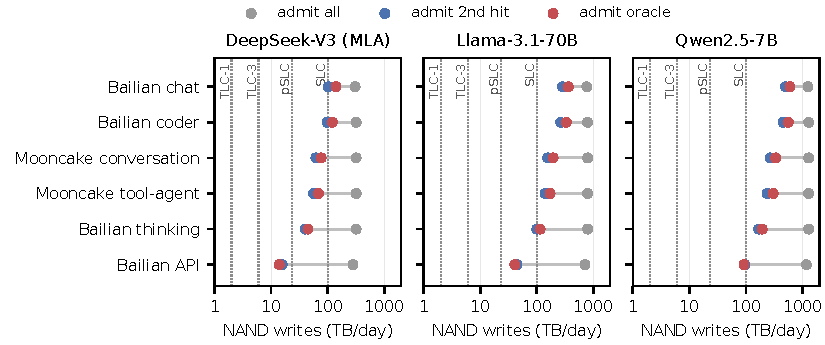
\includegraphics[width=\textwidth]{fig_wear.pdf}
\Description{Bar chart of NAND terabytes written per day per node for each trace, model and admission policy, with horizontal lines for the five-year budgets of TLC, pseudo-SLC and SLC devices.}
\caption{NAND writes per node at full prefill duty, BF16 KV, 28\% over-provisioning, with the
five-year budgets of a 2\,TB device.}
\label{fig:wear}
\end{figure}

Two common shortcuts understate wear. Computing hit rates on a full device and multiplying the
write rate by the node's throughput, without dividing the device by $S$, understates the writes of
small models by up to 1.8 times (Qwen2.5-7B, API trace, oracle admission). Taking write
amplification as 1, as HBF Sucks? does~\cite{hbfsucks}, misses a factor of up to 1.55 on the 2\,TB
device and 1.94 on the pseudo-SLC device at 7\% over-provisioning even for an LRU cache, and of 5.2
for request-scoped KV without TRIM (Section~\ref{sec:waf}).

\section{Write amplification depends on how KV dies}
\label{sec:waf}
Figure~\ref{fig:waf} (left) shows the measured write amplification over all prefix-cache
configurations. The median is 1.00. At 28\% over-provisioning it never exceeds 1.07 on the
2\,TB device and 1.18 on the smaller pseudo-SLC device; at 7\% oracle admission reaches 1.55 on the
2\,TB device and 1.94 on the pseudo-SLC device (second hit: 1.34 and 1.66): the hits it keeps refresh
blocks in the NAND tier's
LRU order, so blocks no longer die in the order they were written.

\begin{figure}[t]
\centering
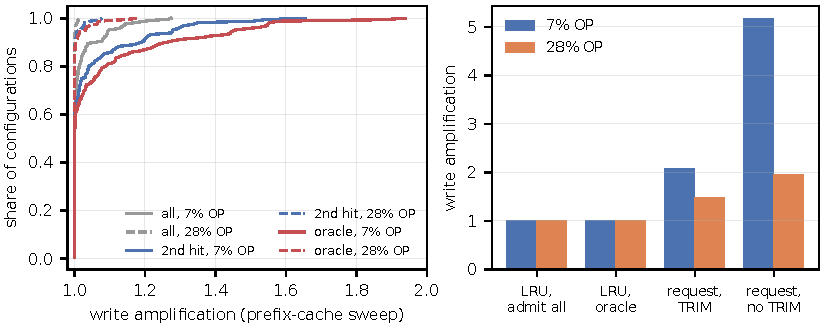
\includegraphics[width=\textwidth]{fig_waf.pdf}
\Description{Left, distribution of measured write amplification over the sweep; right, write amplification for an LRU prefix cache and for request-scoped KV with and without TRIM.}
\caption{Left: distribution of write amplification over the sweep. Right: write amplification by
how KV dies, on the Bailian thinking trace with 64 KV blocks per erase block.}
\label{fig:waf}
\end{figure}

The right panel isolates the cause. An LRU cache evicts blocks roughly in write order, so whole
erase blocks die together and garbage collection copies almost nothing: write amplification 1.00
to 1.02. HiFC reports 1.02 from host-side SMART counters for append-only writes on a consumer
drive~\cite{hifc}. If instead KV is kept per request and freed when the request ends, concurrent requests interleave
their blocks in every erase block and end at different times. This is how a tier behaves when it
holds the KV of live requests rather than a prefix cache: preempted or swapped requests~\cite{vllm},
agent sessions paused on tools, and decode KV of long reasoning requests offloaded while they run;
ScaleFlux names the same pattern, KV invalidated asynchronously across sessions~\cite{scaleflux}.
We model the last case on the Bailian thinking trace (Section~\ref{sec:method}): write amplification is 2.1 at 7\% over-provisioning
with TRIM. CXL.mem has no TRIM, so freed blocks stay valid in the FTL until the host reuses their
addresses, and write amplification rises to 5.2, 2.5 times the TRIM case. HBFlex reports an
average of about 30 for DeepSeek-V4-Pro KV pages of mixed lifetimes sharing HBF erase
blocks~\cite{hbflex}; the mechanism is the same, on a different device, model and mapping
granularity. Lee et al.\ argue for TRIM in CXL memory in general and, with an analytical model
validated in an FTL simulator, estimate a write-amplification cut of up to 19.7\% for Azure VM
traces at 10\% spare space~\cite{trimcxl}; for request-scoped KV the cut is 60\%, because whole
requests die at once. NVMe SSDs can also separate lifetimes with lifecycle-aware placement, which
ScaleFlux reports more than halved write amplification for KV in preliminary
tests~\cite{scaleflux}; SPLASH gives each request its own HBF region and erases it as a
unit~\cite{splash}. Both need control of flash placement that CXL.mem does not give the host. A hybrid CXL
device that stores request-scoped KV therefore needs either generous
over-provisioning or a way for the host to declare data dead, and a serving engine that frees KV
in LRU order avoids the problem.

\section{Telling the device that KV is dead}
\label{sec:discard}
Request-scoped KV wastes flash twice on CXL.mem: dead blocks that device DRAM evicts are written to
NAND, and once there they stay valid until the host reuses their address. The serving engine knows
when a request ends, so it can say so. We evaluate a per-request discard. When a request ends, the
engine sends one command that names the request's blocks; the device drops their copies from its
DRAM without writing them back, trims them in the FTL and acknowledges. The host reuses a block's
address only after the acknowledgment, so a late discard never hits new data, the hazard Lee et al.\
point out for TRIM over CXL.io~\cite{trimcxl}. One command per finished request is a low rate: 1.5
per second on the Bailian thinking trace, and at most about 100 per second when the trace is scaled
to a node ($S \le 67$ in our sweep). The management path (a CXL.io mailbox command) is fast enough
if a command completes in under 10\,ms or covers several requests, and CXL.mem needs no change. Lee
et al.\ propose TRIM as a privileged, asynchronous CXL.io command issued by the operating system or
by applications through a system call, and leave the initiator layer, granularity and frequency
open~\cite{trimcxl}; here the initiator is the serving
engine, and the DRAM drop adds to the trim.

\textbf{Method.} We use the request-scoped stream of Section~\ref{sec:method} with a write-back LRU
DRAM cache of 10\% or 25\% of the peak live KV in front of the FTL (7\% over-provisioning).
Discards queue on one serial channel and take 1\,ms to 10\,s each. After each block it writes, a
request reads 0, 1 or 4 of its earlier blocks at random, as sparse attention over offloaded KV would;
a read that misses DRAM fetches the block from NAND as a clean copy.

\begin{table}[t]
\caption{Flash page programs per KV block written by the host (NAND writes times write
amplification), request-scoped KV on the Bailian thinking trace, 7\% over-provisioning.}
\label{tab:discard}
\small
\begin{tabular}{rrrrrr}
\toprule
DRAM / live KV & reads per write & no discard & 1\,ms & 100\,ms & 1\,s (overloaded) \\
\midrule
10\% & 0 & 5.12 & 1.05 & 1.05 & 2.60 \\
10\% & 1 & 5.20 & 1.28 & 1.28 & 3.01 \\
10\% & 4 & 5.22 & 1.55 & 1.55 & 3.55 \\
25\% & 0 & 4.40 & 0.48 & 0.48 & 1.53 \\
25\% & 1 & 4.84 & 0.63 & 0.63 & 1.83 \\
25\% & 4 & 5.24 & 0.86 & 0.86 & 2.31 \\
\bottomrule
\end{tabular}
\end{table}

\textbf{Results.} With 1 to 100\,ms per command, discards cut flash programs by 3.4 to 9.1 times
(Table~\ref{tab:discard}); the result is the same at 1\,ms and at 100\,ms. Two effects add up.
Dropping dead copies from DRAM cuts NAND writes by 17 to 57\%, more with more DRAM and fewer reads,
and trimming cuts write amplification from 4.9--5.3 to 1.26--1.87. Addresses waiting for an
acknowledgment peak at 3.5\% of the peak live KV, but they peak when live KV is low: with 1\% extra
address space no allocation stalls at 1 to 100\,ms per command. The command channel fails only when completions per second times the command latency
exceed 1: at 1\,s per command and 1.5 completions per second the queue grows without bound, the
host stalls on about 10,000 allocations and the gain falls to 1.5 to 2.9 times. At node scale a
command must therefore take under 10\,ms or cover several requests. On this trace the peak live KV
is 731\,GB for Llama-3.1-70B and 157\,GB for DeepSeek-V3, so 10 to 25\% of it is 16 to 39\,GB of
device DRAM for DeepSeek-V3, within CMM-H's 48\,GB, but 73 to 183\,GB for Llama-3.1-70B. For a
prefix cache, device DRAM changes NAND writes by under 5\% in most cases (Section~\ref{sec:prov});
it saves flash only when the device learns what is dead.

\section{Provisioning}
\label{sec:prov}
Table~\ref{tab:prov} gives the cheapest flash class that lasts five years with second-hit
admission. Four rules follow.
\begin{enumerate}
\item \emph{Admission control is mandatory.} Admit-all never fits TLC, fits pseudo-SLC only for
DeepSeek-V3 with INT4 KV at partial prefill duty (4 of 54 cases), and at full prefill duty fits
nothing in 48 of 54 cases.
\item \emph{Workload decides the flash class.} TLC fits API-like traffic at partial prefill duty
(6 of 9 cases), but reasoning traffic only in 1 of 9 and interactive traffic (chat, coding,
conversation and agent) only in 2 of 36, all DeepSeek-V3 with INT4 KV. Interactive
traffic needs pseudo-SLC or SLC, and 16 of its 36 cases at full prefill duty (and 2 of 36 at partial
duty) exceed even 100\,TB/day.
\item \emph{KV precision is worth about one flash class.} FP8 halves and INT4 quarters the NAND
writes (0.49 and 0.24 times BF16 on average).
\item \emph{Model architecture matters as much as traffic.} With second-hit admission, MLA writes
2.3 to 2.8 times less than a GQA 70B model per node, and small GQA models write the most.
\end{enumerate}
Drives announced for KV caching at 7 to more than 10 DWPD~\cite{scaleflux} would cover, at 10 DWPD
(20\,TB/day on a 2\,TB device), 31 of the 54 cases at partial prefill duty and 9 of 54 at full duty with
second-hit admission; at 7 DWPD, 21 and 4. Using the 1.7 times higher sequential rating for TLC moves 9 of the 108 cases from pseudo-SLC to
TLC; interactive traffic then fits TLC in 6 of 36 cases at partial duty, still all DeepSeek-V3, now
with FP8 or INT4 KV. Pseudo-SLC's smaller capacity (667\,GB) costs little: the median hit share drops
by 1.4 points and the write rate is unchanged in the median. A second wall is bandwidth: 7\% of the
cases (22 of 324) need more than the about 5\,GB/s that the 48\,GB CMM-H sustains once its working
set is much larger than its DRAM cache~\cite{cmmh_hs}, all of them with admit-all or Qwen2.5-7B.

\textbf{Device DRAM size.} Growing the device's DRAM cache from 16 to 256\,GB (Bailian API, chat
and thinking traces, Llama-3.1-70B and DeepSeek-V3, BF16, full duty, second-hit and oracle
admission) changes the NAND writes by $-32$ to $+6\%$, and by under 5\% in most cases, while the
share of hits served from DRAM rises from 0.24--0.49 to 0.35--0.90. A larger DRAM cache improves hit
latency but not lifetime: in a node serving many users, a block's reuse arrives long after it has
left any affordable DRAM cache.

\begin{table}[t]
\caption{Cheapest flash class that lasts five years with second-hit admission, by prefill duty and
KV precision. TLC-1/TLC-3: TLC at 1/3 DWPD; none: above 100\,TB/day.}
\label{tab:prov}
\resizebox{\textwidth}{!}{\begin{tabular}{llllllll}
\toprule
trace & model & 100\% BF16 & 100\% FP8 & 100\% INT4 & 30\% BF16 & 30\% FP8 & 30\% INT4 \\
\midrule
Bailian API & DeepSeek-V3 & pSLC & pSLC & TLC-3 & TLC-3 & TLC-3 & TLC-1 \\
Bailian API & Llama-3.1-70B & SLC & SLC & pSLC & pSLC & TLC-3 & TLC-3 \\
Bailian API & Qwen2.5-7B & SLC & SLC & pSLC & SLC & pSLC & TLC-3 \\
Bailian thinking & DeepSeek-V3 & SLC & pSLC & pSLC & pSLC & pSLC & TLC-3 \\
Bailian thinking & Llama-3.1-70B & none & SLC & SLC & SLC & pSLC & pSLC \\
Bailian thinking & Qwen2.5-7B & none & SLC & SLC & SLC & SLC & pSLC \\
Mooncake tool-agent & DeepSeek-V3 & SLC & SLC & pSLC & pSLC & pSLC & TLC-3 \\
Mooncake tool-agent & Llama-3.1-70B & none & SLC & SLC & SLC & pSLC & pSLC \\
Mooncake tool-agent & Qwen2.5-7B & none & none & SLC & SLC & SLC & pSLC \\
Mooncake conversation & DeepSeek-V3 & SLC & SLC & pSLC & pSLC & pSLC & TLC-3 \\
Mooncake conversation & Llama-3.1-70B & none & SLC & SLC & SLC & pSLC & pSLC \\
Mooncake conversation & Qwen2.5-7B & none & none & SLC & SLC & SLC & pSLC \\
Bailian coder & DeepSeek-V3 & SLC & SLC & SLC & SLC & pSLC & pSLC \\
Bailian coder & Llama-3.1-70B & none & none & SLC & SLC & SLC & pSLC \\
Bailian coder & Qwen2.5-7B & none & none & SLC & none & SLC & SLC \\
Bailian chat & DeepSeek-V3 & none & SLC & SLC & SLC & pSLC & pSLC \\
Bailian chat & Llama-3.1-70B & none & none & SLC & SLC & SLC & pSLC \\
Bailian chat & Qwen2.5-7B & none & none & none & none & SLC & SLC \\
\bottomrule
\end{tabular}
}
\end{table}

\section{When does loading beat recomputing?}
\label{sec:load}
A hit served from the device pays only if loading the KV is faster than recomputing it. Recomputing
$n$ tokens on the node takes $t(n) = (2Pn + Lwn^2)/(G F u)$, with $w$ the attention width; loading
takes $n b / B$ for $b$ bytes of KV per token over a path of $B$ bytes per second. The break-even
bandwidth $B^* = nb/t(n)$ (Figure~\ref{fig:load}) falls with context length because attention makes
recompute superlinear; the trade-off itself is formalized in~\cite{restore_recompute,pykvcache}.
On 8 H100 GPUs, hits served from the device's DRAM cache (about 27\,GB/s~\cite{cmmh_hs}) always
pay. Hits from NAND (about 5\,GB/s) pay for DeepSeek-V3 at every precision, for Llama-3.1-70B only
with FP8 or INT4 KV, and for Qwen2.5-7B only with INT4. On B200 GPUs the break-even rises 2.3 times;
NAND hits then pay only for DeepSeek-V3 with FP8 or INT4 KV (BF16 only at 32K tokens) and for
Llama-3.1-70B with INT4 KV at 8K and 32K tokens. Lower KV precision thus helps twice: it cuts writes and
makes NAND hits worth serving.

\begin{figure}[t]
\centering
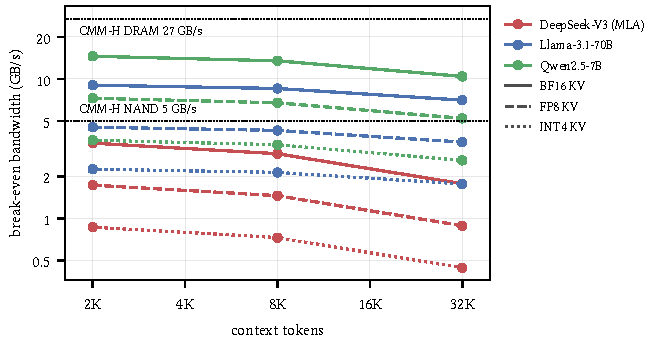
\includegraphics[width=0.75\textwidth]{fig_load.pdf}
\Description{Break-even load bandwidth versus context length for each model and KV precision on H100 and B200 nodes, with horizontal lines for the device's DRAM and NAND bandwidth.}
\caption{Bandwidth above which loading KV beats recomputing it on 8 H100 GPUs, with measured
device bandwidths.}
\label{fig:load}
\end{figure}

\section{Shared pool or per-host caches?}
\label{sec:pool}
A CXL pool shared by several prefill hosts holds each block once and serves every host; per-host
caches duplicate popular blocks. Figure~\ref{fig:pool} compares a pool with per-host caches under
random and cache-aware routing; cache-aware routing sends a request to the host with the longest
cached prefix unless that host's load exceeds the mean by more than 25\%. Over 4 to 16 hosts and
total capacities of 2 to 50\% of the unique blocks, the pool hits 1.05 to 4.5 times as often as
random routing and writes 1.03 to 1.9 times fewer blocks, but beats cache-aware routing by only
1 to 18\% in hits and 1 to 9\% in writes. Mooncake reports up to 136\% more hits for its global
pool than for per-node local caches with prefix-aware routing, on 10 prefill nodes of 3M tokens
each~\cite{mooncake}. Reproducing that
setup, the pool gains 3 to 10\% when the scheduler allows 5 to 100\% imbalance, 15 to 43\% when it
balances exactly and up to 165\% when it ignores load (Figure~\ref{fig:pool}, right). The value of
a pool therefore depends mostly on how strictly the scheduler balances load, which also bounds what
a pooled CXL tier saves in wear.

\begin{figure}[t]
\centering
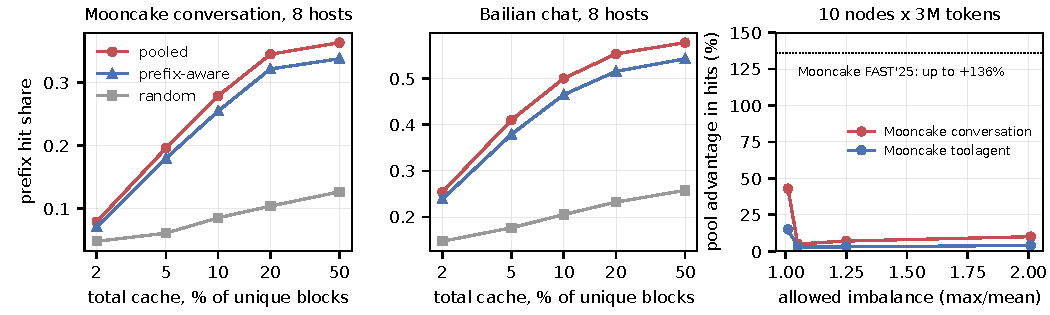
\includegraphics[width=\textwidth]{fig_pool.pdf}
\Description{Prefix hit share of a shared pool versus per-host caches under random and cache-aware routing, and the pool's advantage as the allowed load imbalance varies.}
\caption{Prefix hit share of a shared pool and of per-host caches (8 hosts), and the pool's
advantage at Mooncake's scale as the scheduler's allowed imbalance varies.}
\label{fig:pool}
\end{figure}

\section{Discussion and limitations}
\textbf{Scaling.} Modeling a node as $S$ interleaved copies of a trace assumes independent users;
real routing can concentrate a conversation on one node, which shortens reuse distances and favors
the cache. The traces cover one to two hours, so daily cycles are not represented.

\textbf{Write amplification.} Our FTL matches closed forms and MQSim but not a specific drive; a
quarter of the 2\,TB cases and a tenth of the pseudo-SLC cases are too short to reach steady state
and use write amplification 1, and in 15\% only one KV block fits in an erase block. Devices with
large superblocks or internal DRAM write coalescing will differ.

\textbf{Retention.} KV needs minutes to hours of retention, not the months that enterprise ratings
assume; relaxing internal retention from three years to three days could raise MLC endurance by up
to 50 times, extrapolated from characterization data~\cite{warm}. A hybrid CXL device that knew its
contents were KV could trade retention for endurance; with second-hit admission, a tenfold gain
would move 22 of the 34 interactive cases that need SLC to TLC. We leave this to future work.

\textbf{Related work.} Endurance of flash KV tiers has been studied for HBF: HBF
Sucks?~\cite{hbfsucks}, the endurance letters of Son et al.~\cite{son_hbf} and Kyung
et al.~\cite{kyung_hbf}, HBFlex (lifetime-aware block packing)~\cite{hbflex}, Lachesis (lifetime-aware
HBM/HBF placement)~\cite{lachesis}, LRU-K admission for recommendation KV~\cite{huawei_hbf},
request admission~\cite{berkeley_hbf}, SPLASH (per-request regions)~\cite{splash}, and HiFC with
pseudo-SLC on a consumer SSD~\cite{hifc}. Lee et al.\ argue for TRIM in CXL memory and model it on
VM workloads~\cite{trimcxl}. Hybrid CXL KV systems evaluate performance without
wear~\cite{hymcache,itme,lmcxd,tempokv}; CMM-H has been characterized~\cite{cmmh,cmmh_hs} and
emulated~\cite{cylon}. KVCache-in-the-Wild characterizes KV reuse in production~\cite{kvwild}, and
Mooncake and TokenLake pool KV across nodes~\cite{mooncake,tokenlake}. We add the hybrid device
model, consistent per-node scaling, measured write amplification including the no-TRIM case,
provisioning across flash type, KV precision, admission and prefill duty, and a discard mechanism,
and we show that the way the serving engine frees KV matters more than the device's
over-provisioning.

\textbf{Implications.} For serving engines: keep KV on a hybrid device as an LRU prefix cache, or
send a discard when request-scoped KV dies, and admit only reused blocks. For device
designers: a way for the host to declare data dead, such as TRIM for CXL memory~\cite{trimcxl},
together with dropping the dead data from device DRAM, is worth 3.4 to 9.1 times in flash writes for
request-scoped KV (Section~\ref{sec:discard}), and
relaxed retention could move interactive traffic to cheaper flash. For operators: the provisioning
rules of Section~\ref{sec:prov} pick the flash class from the traffic type, KV precision and
prefill duty.

\section{Conclusion}
How KV dies decides how flash wears. An LRU KV cache on a hybrid CXL device keeps write
amplification near 1, while request-scoped KV on CXL.mem, which has no TRIM, raises it to 5.2.
Even near 1, the write rate itself is the wall: with second-hit admission a hybrid device lasts five
years on TLC flash in only 10 of 108 cases, mostly API-like traffic at partial prefill duty and
4-bit MLA KV at partial duty. Interactive traffic needs pseudo-SLC or SLC, or a device that trades retention for endurance.
Admission control and lower KV precision are the cheapest levers, and for request-scoped KV a
discard per finished request cuts flash writes 3.4 to 9.1 times.

\bibliographystyle{ACM-Reference-Format}
\bibliography{p2}

\end{document}
